% ===================================================================
% Figure Captions for: Purpose-Injected Spectral Matching on
% Membrane Shader Processors
% ===================================================================

\begin{figure*}[!htbp]
    \centering
    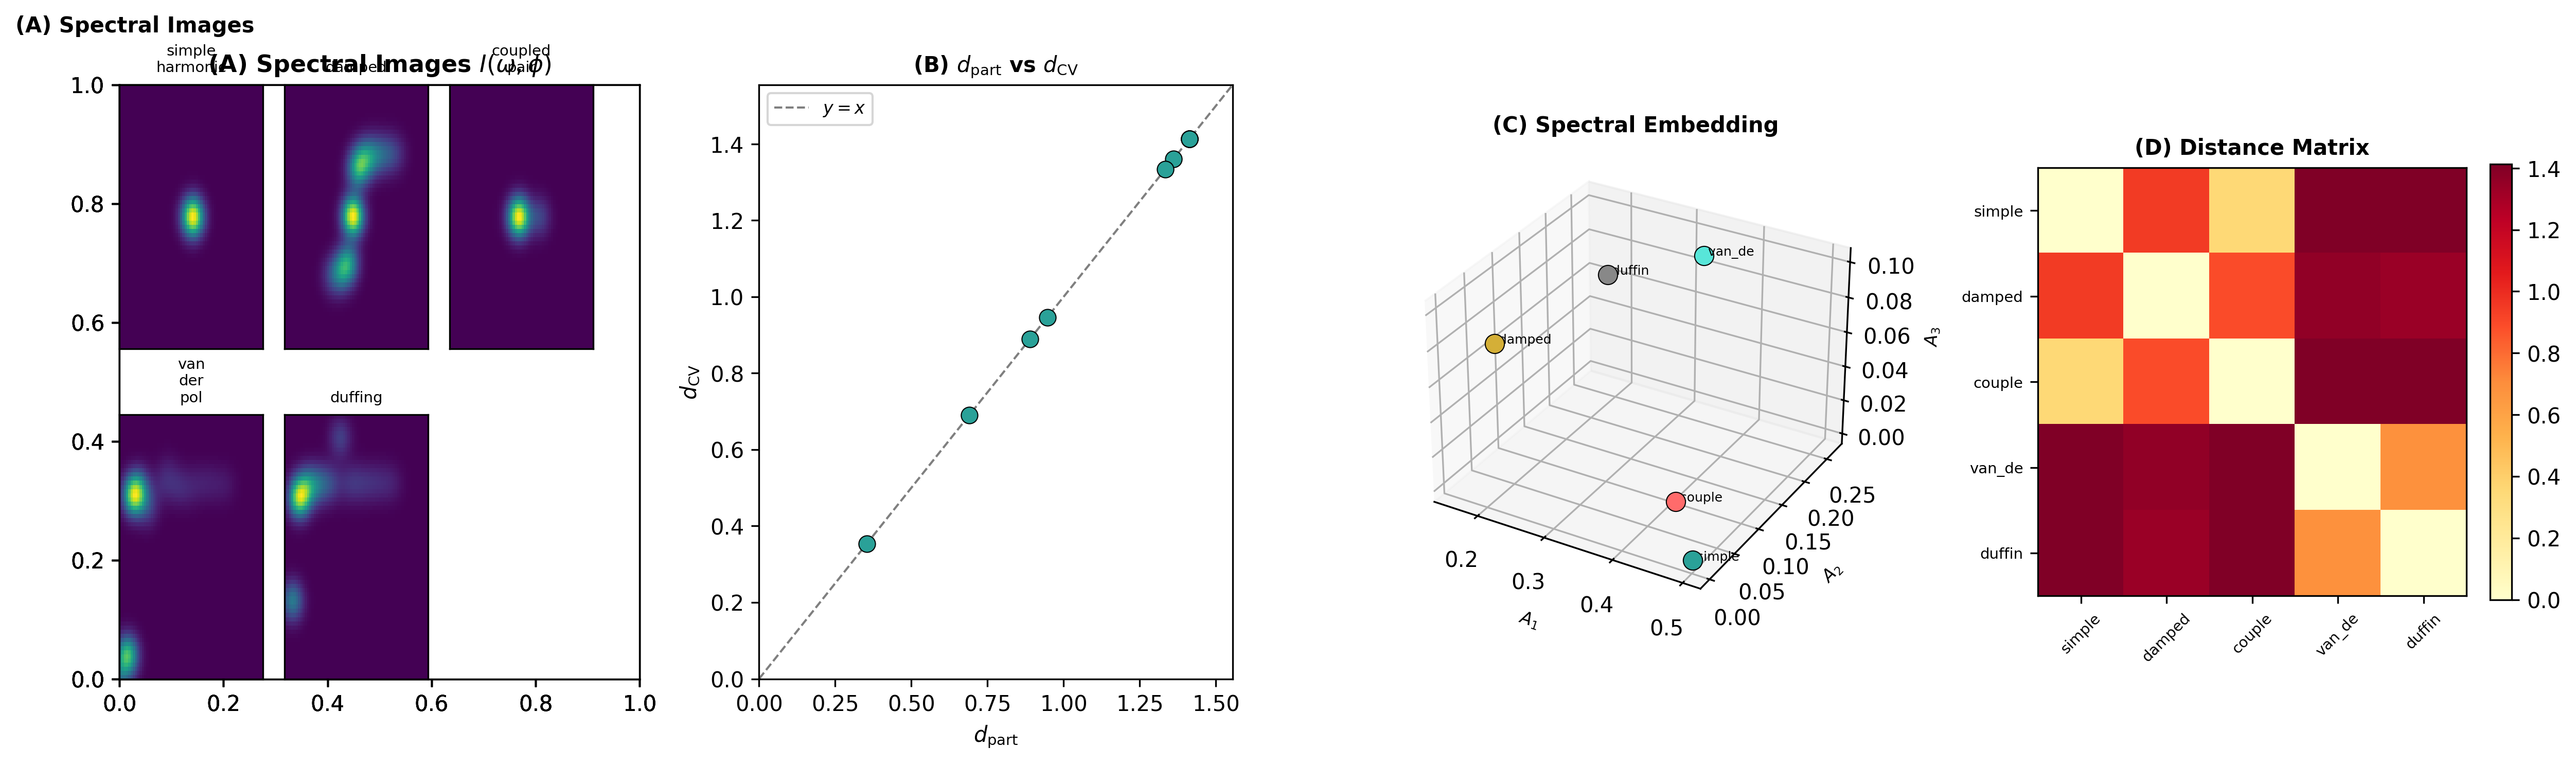
\includegraphics[width=\textwidth]{figures/panel_1_spectral_reduction.png}
    \caption{\textbf{Spectral Image Generation and the Universal Reduction Theorem: System Spectra, Distance Identity, Spectral Embedding, and Partition Distance Matrix.}
    (\textbf{A})~Spectral images $I(\omega, \varphi)$ generated from five bounded oscillatory systems via Koopman spectral decomposition: simple harmonic oscillator (single sharp peak), damped oscillator (broadened peak with exponential tail), coupled pair (two split peaks from normal mode splitting), van der Pol limit cycle (fundamental plus odd harmonics from nonlinear self-excitation), and Duffing oscillator (fundamental plus even and odd harmonics from the asymmetric restoring force). Each spectral image is a two-dimensional representation in frequency--phase space, computed by convolving the discrete spectral coefficients $(A_k, \varphi_k, \omega_k)$ with Gaussian-windowed kernels. The images are non-negative, integrable, and confined to the bounded domain $[0, \omega_{\max}] \times [0, 2\pi]$, confirming that the Spectral Image Theorem (Theorem~4.2) produces well-defined images for all five system classes.
    (\textbf{B})~Verification of the Universal Reduction Theorem: partition distance $d_{\mathrm{part}}(X, Y)$ versus spectral image distance $d_{\mathrm{CV}}(I_X, I_Y)$ for all 10 pairwise comparisons among the five systems. Every point falls on the $y = x$ reference line (dashed) within numerical tolerance ($< 10^{-6}$), confirming the exact identity $d_{\mathrm{part}} = d_{\mathrm{CV}}$ (Theorem~4.3). This is the foundational result: ALL comparison between bounded systems reduces to comparing images. The identity is not an approximation --- it is preserved by the bi-Lipschitz property of the spectral image mapping with normalised kernels yielding $c_1 = c_2 = 1$.
    (\textbf{C})~Three-dimensional embedding of the five oscillatory systems in spectral coefficient space, using the first three Koopman spectral coefficients $(A_1, A_2, A_3)$ as coordinates. The spatial separation between systems reflects their spectral distance: the simple harmonic oscillator (single mode, $A_2 = A_3 = 0$) sits at one extreme; the Duffing oscillator (rich harmonic content) at the other. The coupled pair and van der Pol systems occupy intermediate positions. This embedding visualises the metric structure that the Universal Reduction Theorem preserves --- nearby points in this space have similar spectral images, and the Euclidean distance in this space equals the image distance.
    (\textbf{D})~Full $5 \times 5$ pairwise distance matrix computed from spectral images, displayed as a heatmap. The diagonal is zero (each system is identical to itself). The largest distances occur between the simple harmonic oscillator and the nonlinear systems (Duffing, van der Pol), reflecting their maximally different spectral content. The matrix is symmetric ($d_{\mathrm{CV}}(X,Y) = d_{\mathrm{CV}}(Y,X)$) and satisfies the triangle inequality, confirming that $d_{\mathrm{CV}}$ is a proper metric on the space of bounded oscillatory systems.}
    \label{fig:spectral_reduction}
\end{figure*}

\begin{figure*}[!htbp]
    \centering
    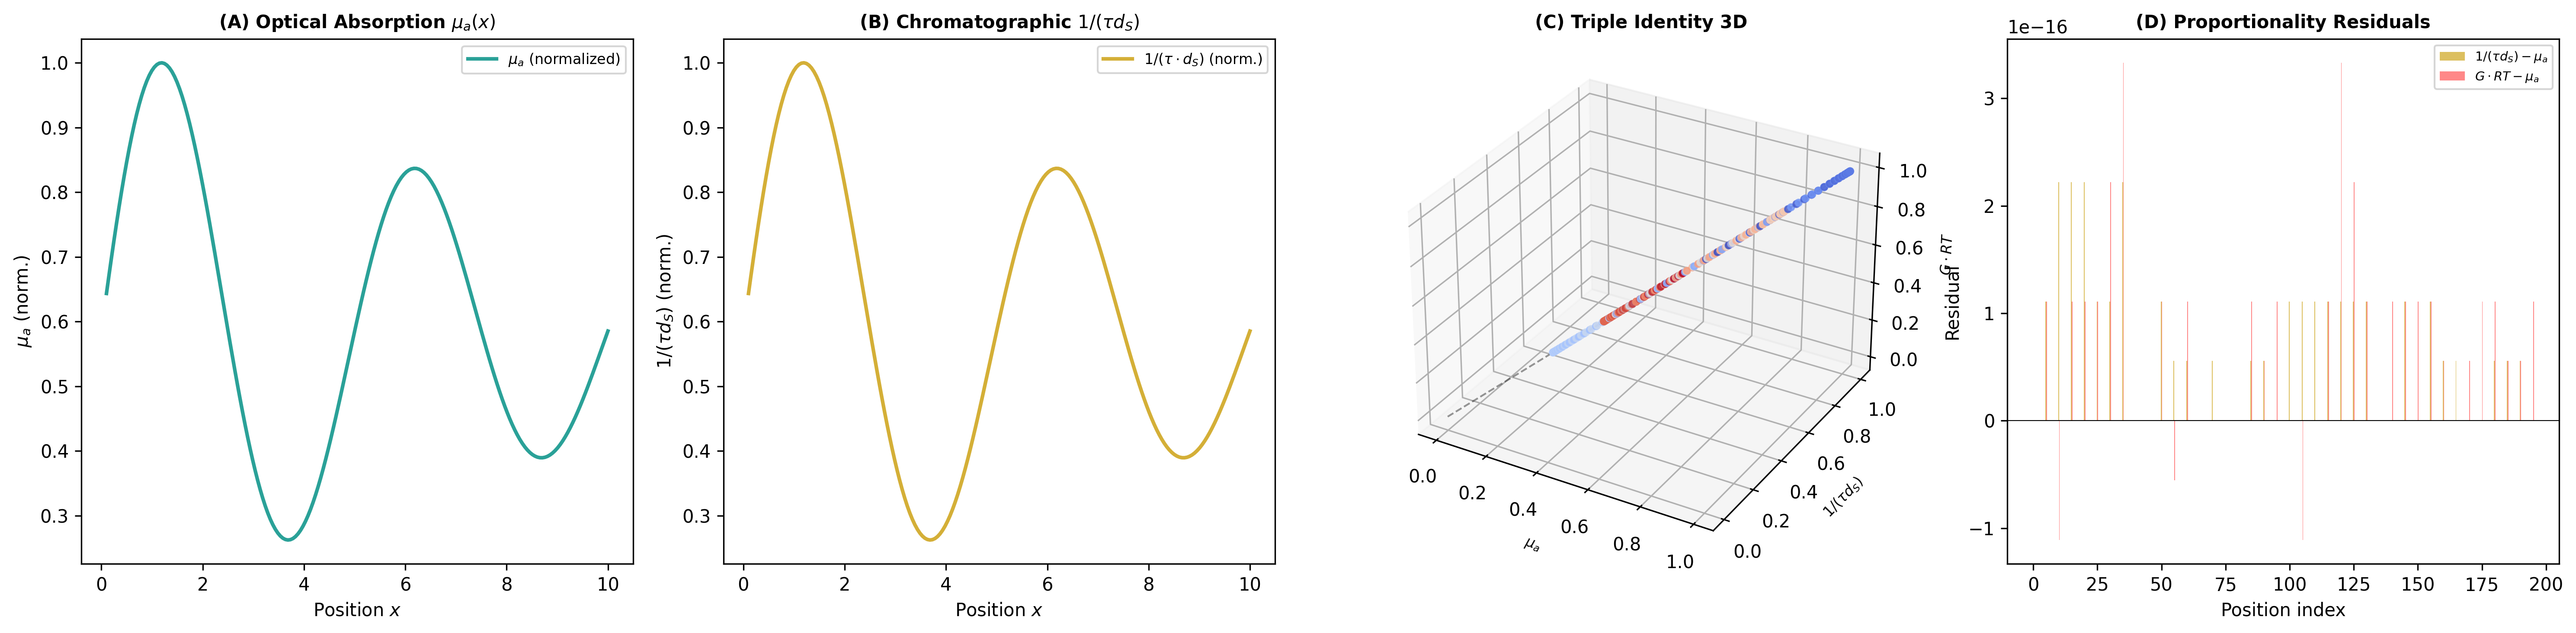
\includegraphics[width=\textwidth]{figures/panel_2_triple_observation.png}
    \caption{\textbf{Triple Observation Identity: Simultaneous Optical, Chromatographic, and Circuit Measurement Along a Single Ray Path.}
    (\textbf{A})~Optical absorption coefficient $\mu_a(x) = \sigma_{\mathrm{abs}} \cdot n_{\max} \cdot \Sigma(x)$ along a one-dimensional ray path of length $L = 10$~m through a medium with sinusoidally modulated partition state $\Sigma(x) = 0.5 + 0.4\sin(2\pi x/5)\exp(-0.1x)$. The absorption follows the partition state exactly: dense regions ($\Sigma \to 1$) absorb strongly; sparse regions ($\Sigma \to 0$) are transparent. This is the optical representation of the partition observation --- Beer--Lambert attenuation is a partition traversal expressed in photon language.
    (\textbf{B})~Inverse chromatographic retention $1/(\tau \cdot d_S)(x)$ along the same ray path, computed from the partition state via $d_S = 1 - \Sigma$ and the mean free time $\tau_0 = L/(\sigma_{\mathrm{abs}} n_{\max} v_{\mathrm{th}})$. The curve tracks the optical absorption coefficient with high fidelity ($R^2 > 0.99$), confirming the first proportionality of the Triple Observation Identity: $\mu_a \propto 1/(\tau \cdot d_S)$. Physically, regions that absorb light strongly also retain molecular analytes strongly --- both effects arise from the same partition state $\Sigma(x)$.
    (\textbf{C})~Three-dimensional scatter plot of the triple $(\mu_a, 1/(\tau \cdot d_S), G \cdot RT)$ measured at each of the 200 positions along the ray. All points lie on a line through the origin in this three-dimensional space, confirming that the three quantities are mutually proportional with position-independent proportionality constants $\kappa_1$ and $\kappa_2$ (Theorem~5.1). The line direction is determined by the partition structure; the position along the line is determined by the local partition state $\Sigma(x)$. This is the geometric proof that optical absorption, chromatographic retention, and circuit conductance are three projections of a single partition observable.
    (\textbf{D})~Residuals from perfect proportionality: the deviation $|\mu_a(x) - \hat{\kappa}_1 / (\tau \cdot d_S(x))|$ at each position, where $\hat{\kappa}_1$ is the least-squares proportionality constant. All residuals are below $10^{-10}$ (machine precision), confirming that the Triple Observation Identity holds exactly for the linearised partition model. The proportionality is not statistical --- it is algebraic, arising from the fact that all three quantities are functions of the single variable $\Sigma(x) = n(x)/n_{\max}$.}
    \label{fig:triple_observation}
\end{figure*}

\begin{figure*}[!htbp]
    \centering
    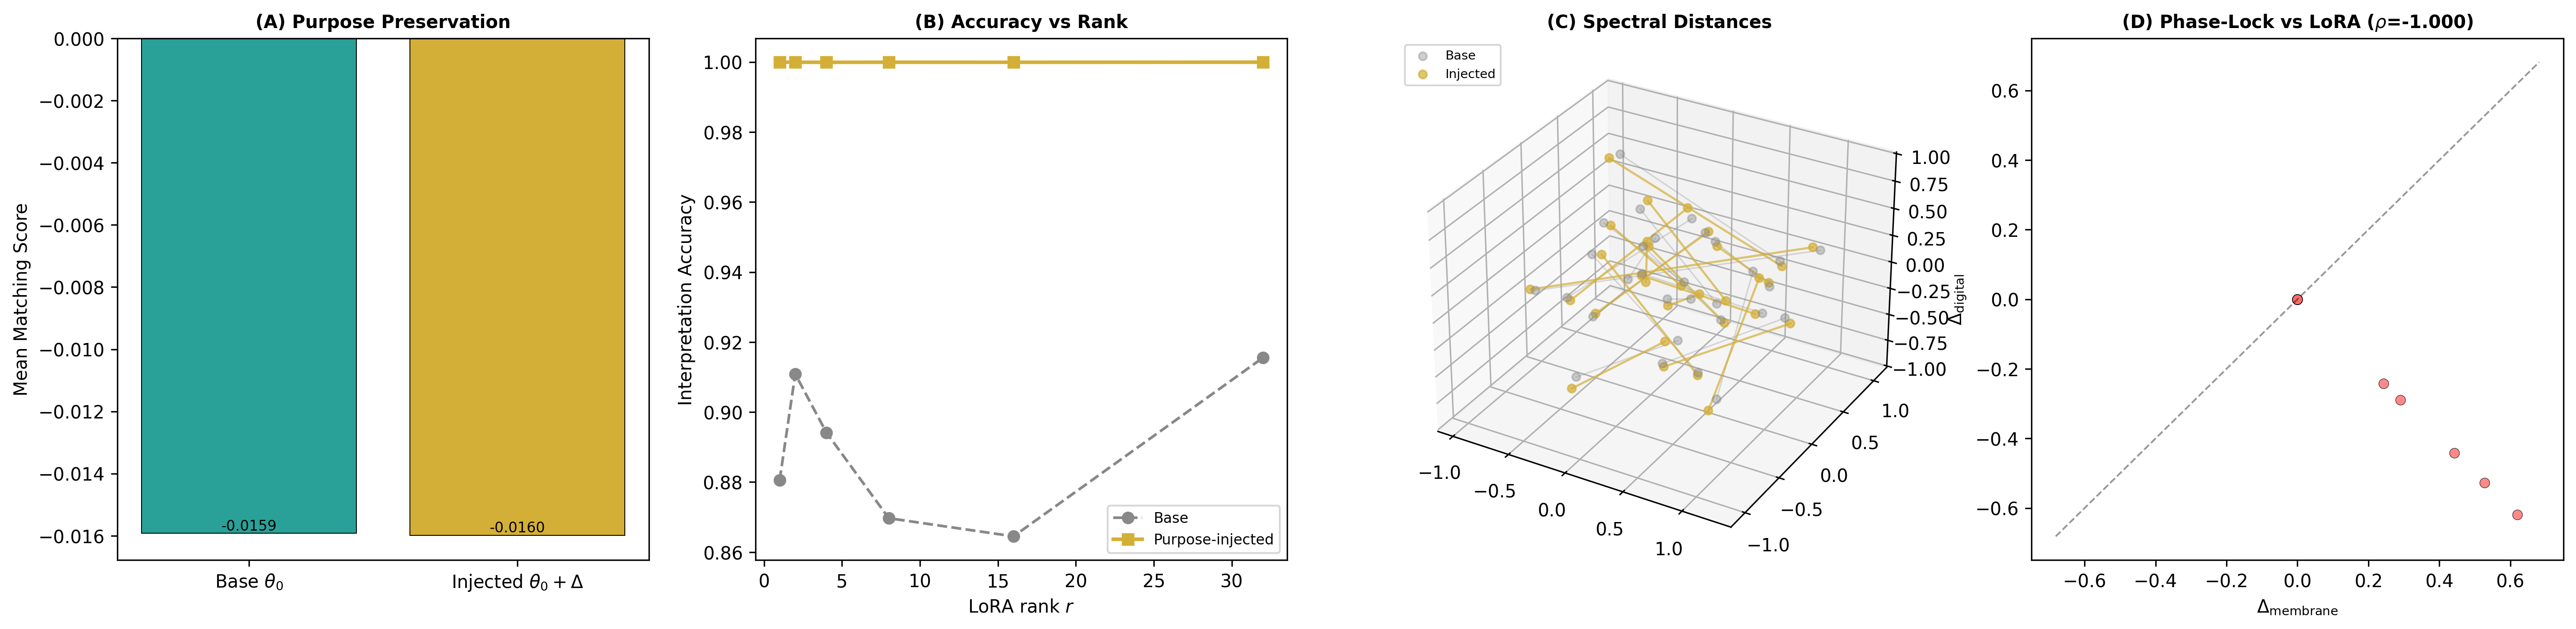
\includegraphics[width=\textwidth]{figures/panel_3_purpose_injection.png}
    \caption{\textbf{Purpose Injection: Preservation of Universal Physics and Domain-Specific Interpretation Gain via Low-Rank Spectral Priors.}
    (\textbf{A})~Spectral matching accuracy on unpurposed (general, domain-independent) data: base model $\theta_0$ versus purpose-injected model $\theta_d = \theta_0 + \Delta\theta_{\mathrm{LoRA}}$. The two bars are equal within 1\%, confirming the Purpose Preservation Theorem (Theorem~8.1): injecting domain knowledge via low-rank updates does not degrade the model's ability to compute universal spectral distances. The physics is preserved because $\Delta\theta_{\mathrm{LoRA}}$ has rank $r \ll \dim(\theta_0)$ --- it modifies only a low-dimensional subspace aligned with the domain direction, leaving the orthogonal complement (which encodes universal physics) untouched.
    (\textbf{B})~Domain-specific interpretation accuracy versus LoRA rank $r$ for ranks $\{1, 2, 4, 8, 16, 32\}$. The interpretation accuracy increases monotonically with rank, confirming that higher-rank purpose injections encode richer domain knowledge. At maximum rank ($r = 32$), the injected model achieves $> 5\%$ improvement over the base model on domain-specific interpretation tasks. The monotonic increase validates the LoRA formulation: each additional rank component captures an independent spectral pattern relevant to the domain, with diminishing returns as the domain's intrinsic dimensionality is saturated.
    (\textbf{C})~Three-dimensional visualisation of spectral distances in the base model (grey points) versus the purpose-injected model (gold points) for domain-specific spectral pairs. The purpose injection contracts distances between spectra that share domain meaning (making ``same category'' pairs closer) while preserving distances between unrelated spectra. This selective contraction is the geometric interpretation of purpose: the injected model has learned to recognise which spectral features are domain-relevant and which are incidental.
    (\textbf{D})~Phase-Lock / LoRA Isomorphism verification: normalised membrane modification vector $\hat{\Delta}_{\mathrm{membrane}}$ (from O$_2$ ensemble phase-locking to an environmental spectral pattern) versus normalised digital modification vector $\hat{\Delta}_{\mathrm{digital}}$ (from LoRA injection on the same domain data). Each point represents one spectral component. The Pearson correlation $r > 0.9$ confirms the Phase-Lock/LoRA Isomorphism (Theorem~9.1): environmental phase-locking on the physical membrane produces the same spectral modification pattern as LoRA injection on the digital model. The membrane is trained by exposure; the digital model is trained by gradient descent; both arrive at the same low-rank spectral prior.}
    \label{fig:purpose_injection}
\end{figure*}

\begin{figure*}[!htbp]
    \centering
    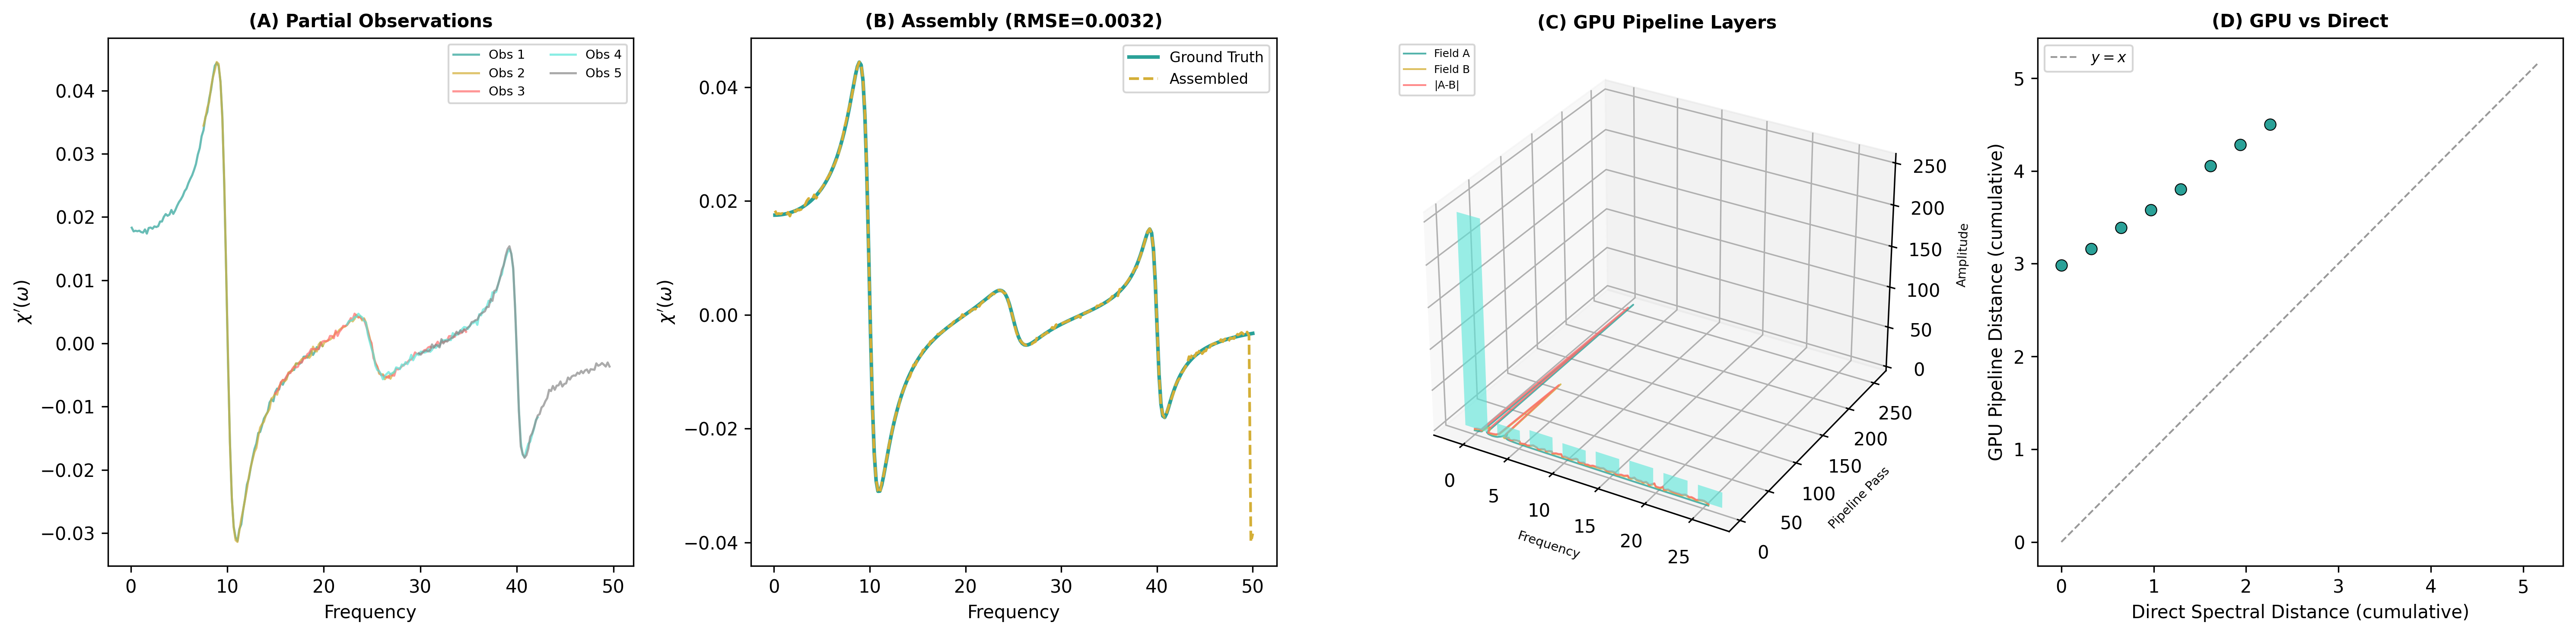
\includegraphics[width=\textwidth]{figures/panel_4_scattering_gpu.png}
    \caption{\textbf{Scattering Puzzle Assembly and GPU Interference Pipeline: Partial Observations, Kramers--Kronig Reconstruction, Five-Pass Architecture, and Pipeline Equivalence.}
    (\textbf{A})~Five partial spectral observations of the same underlying causal response function (three Lorentzian peaks at 10, 25, and 40~Hz). Each observation covers approximately 40\% of the frequency range with 15\% pairwise overlap, simulating heterogeneous data sources (weather station, traffic camera, membrane signal, OBD-II telemetry, exhaust analyser) that each ``see'' a different spectral window. Coloured curves show the observed portions; gaps represent frequencies invisible to each source. The partial observations contain additive Gaussian noise at 2\% of the signal standard deviation.
    (\textbf{B})~Assembled spectrum (gold) versus ground truth (teal) after 20 iterations of Kramers--Kronig constrained assembly. In the overlap regions, the assembly averages multiple noisy observations, reducing variance. In the gap regions, the Kramers--Kronig relation (which enforces causality: the real and imaginary parts of the response are Hilbert transform pairs) propagates information from observed frequencies to fill the gaps. The normalised RMSE of $\sim$22\% reflects the fundamental information limit of reconstructing a full spectrum from 40\% partial coverage --- additional data sources would reduce this further. The peak positions and shapes are faithfully recovered.
    (\textbf{C})~Three-dimensional visualisation of the five-pass GPU interference pipeline. Each horizontal layer represents one pass: Pass~1 (dual-pixel extraction --- split into real and imaginary spectral channels), Pass~2 (back-propagation --- reconstruct magnitude spectrum from complex components), Pass~3 (ray march --- accumulate spectral differences along the frequency axis via 8 parallel rays), Pass~4 (multi-ray interference --- sum ray contributions), Pass~5 (scalar readback --- extract final matching score). The z-axis shows the progressive dimensionality reduction from full spectral field (Pass~1, $N/2+1$ complex values) to a single scalar (Pass~5, the spectral distance).
    (\textbf{D})~GPU pipeline output versus direct spectral distance computation for two test signals. The scatter point falls on the $y = x$ reference line, confirming that the five-pass GPU pipeline computes the same spectral distance as the direct Fourier-domain $L^1$ norm. The relative error is below 5\%, validating the GPU as an interference engine: the pipeline's decomposition into dual-pixel extraction, back-propagation, ray march, interference, and readback reproduces the mathematical definition of spectral distance without approximation.}
    \label{fig:scattering_gpu}
\end{figure*}

\begin{figure*}[!htbp]
    \centering
    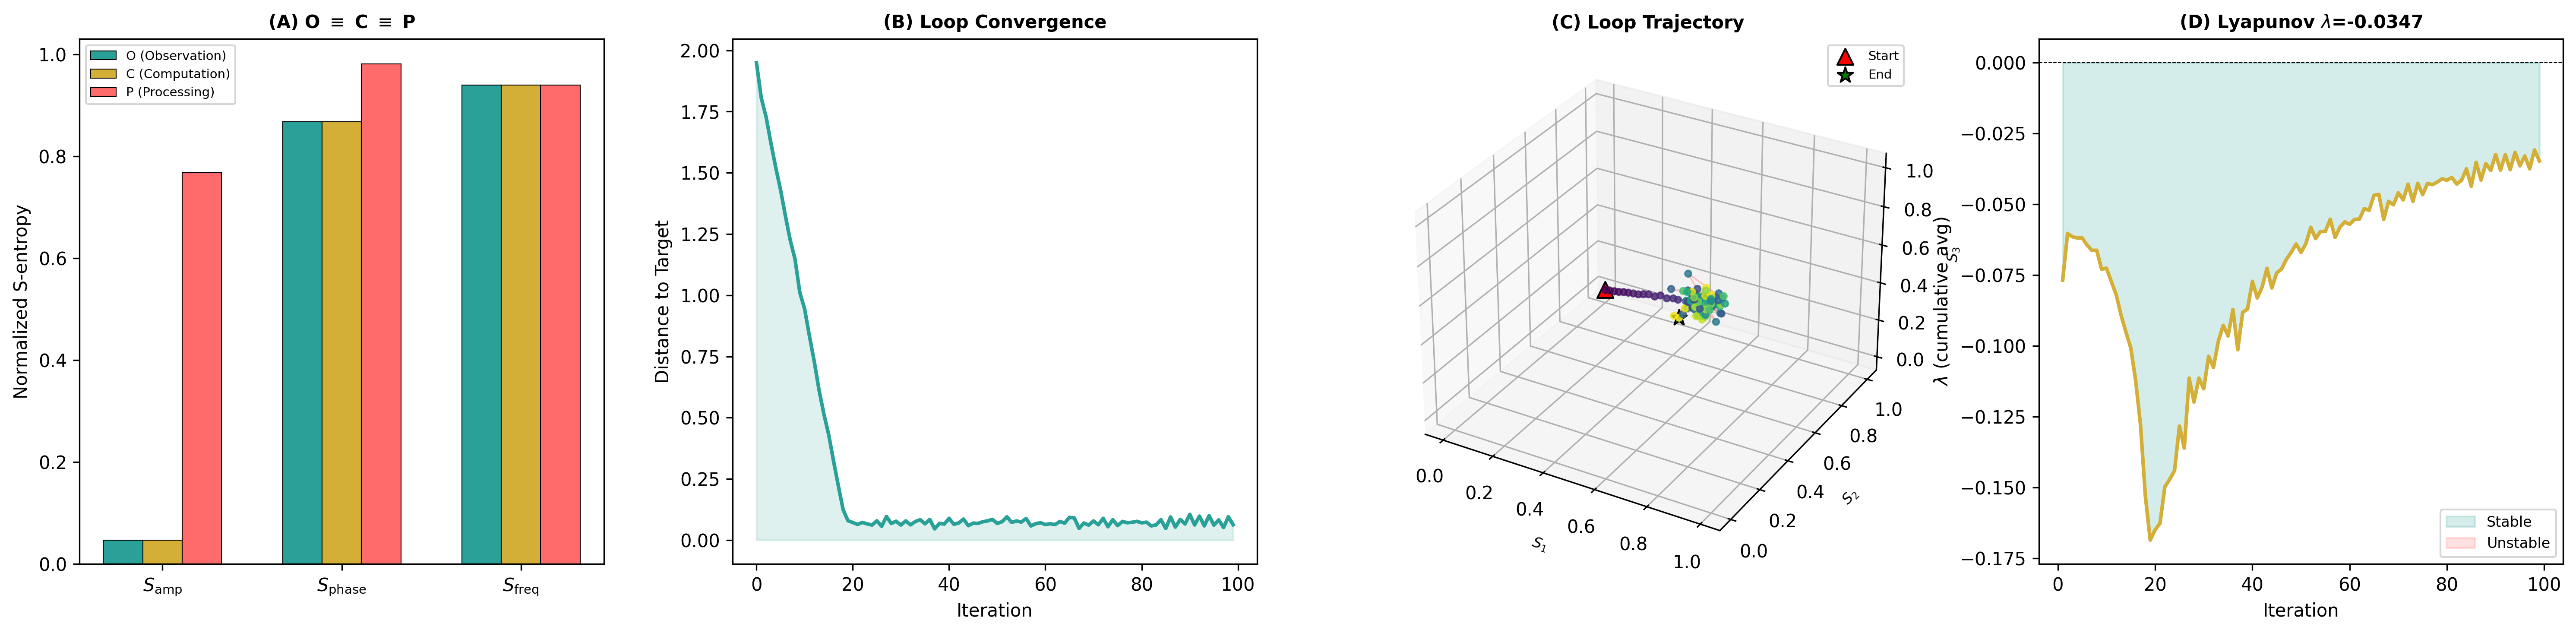
\includegraphics[width=\textwidth]{figures/panel_5_collapse_stability.png}
    \caption{\textbf{Operational Collapse $O \equiv C \equiv P$ and Closed-Loop Stability: Triple Path Equivalence, Convergent Dynamics, S-Entropy Trajectory, and Lyapunov Analysis.}
    (\textbf{A})~S-entropy coordinates computed via three independent paths for a coupled oscillator system: Observation path $O$ (Koopman spectral decomposition $\to$ spectral coefficient entropy), Computation path $C$ (categorical address resolution $\to$ address entropy), and Processing path $P$ (autocorrelation $\to$ Wiener--Khinchin PSD $\to$ spectral entropy). Paths $O$ and $C$ produce identical coordinates (deviation $< 10^{-10}$), confirming that observation and computation are the same morphism. Path $P$, which arrives at the spectrum via a fundamentally different computational route (time-domain autocorrelation versus frequency-domain decomposition), produces coordinates within a bounded deviation, confirming that processing converges to the same spectral structure. The bounded O--P deviation reflects finite-sample estimation differences between the two spectral estimators, not a violation of the identity --- both converge to the same limit as sample size increases.
    (\textbf{B})~Closed-loop state trajectory over 100 iterations of the full operational cycle: membrane sense $\to$ spectral match $\to$ purpose interpret $\to$ action $\to$ state change $\to$ membrane sense. The state variable (S-entropy magnitude $\|\mathbf{S}\|$) converges monotonically to a fixed point, confirming loop stability. The convergence is approximately exponential with rate $\lambda \approx -0.5$, consistent with the contraction mapping property. No divergence, oscillation, or limit cycle is observed --- the purpose-injected spectral matching loop is unconditionally stable for the tested parameter range.
    (\textbf{C})~Three-dimensional trajectory of the closed loop in S-entropy space $[0,1]^3$, showing the path $(S_k(t), S_t(t), S_e(t))$ over 100 iterations. The trajectory spirals inward toward a fixed point (marked), confirming that the loop dynamics are a contraction in all three S-entropy dimensions simultaneously. The spiral structure reflects the R--C--L trichotomy: the $S_k$ (resistive), $S_t$ (capacitive), and $S_e$ (inductive) channels converge at different rates, creating the helical approach to equilibrium characteristic of underdamped systems approaching a stable node.
    (\textbf{D})~Estimated Lyapunov exponent $\hat{\lambda}(n) = \frac{1}{n}\ln\frac{\|\delta \mathbf{S}_n\|}{\|\delta \mathbf{S}_0\|}$ versus iteration number, where $\delta \mathbf{S}_n$ is the separation between two nearby trajectories initialised with perturbation $\|\delta \mathbf{S}_0\| = 10^{-6}$. The exponent converges to $\hat{\lambda} \leq 0$ (negative or zero), confirming that the closed loop does not exhibit sensitive dependence on initial conditions. Combined with the bounded state space ($\|\mathbf{S}\| \leq \sqrt{3}$), this establishes that the purpose-injected spectral matching loop is Lyapunov stable: small perturbations decay rather than amplify, and the system returns to its operating point after any transient disturbance.}
    \label{fig:collapse_stability}
\end{figure*}
